\documentclass[twoside,english, a4paper]{article}
\usepackage{graphicx}
\usepackage{amssymb,amsmath}

\newcommand{\mathbox}[1]{\fbox{\begin{minipage}{\linewidth}#1\end{minipage}}}
%~ \newcommand{\mathbox}[1]{#1}

\title{\textsc{Dnssec} Key State Transitions \\ \small The Grand Unified Theory of Everything \textsc{Dnssec} ;)}
\author{Yuri Schaeffer, Yuri@NLnetLabs.nl}
\date{\today}

\begin{document}
\maketitle
\tableofcontents

\section{Introduction}

During a key roll over each involved key has a state. Matthijs 
Mekking pointed out that the state-machine for this key can be 
represented as three individual smaller state machines: The state at 
the parent, the private key state, and the public key state. 

That idea is the basis for this document. A cache centered rather 
than a roll-over centered approach is chosen and the three different 
state machines are generalized to one type of state machine. The three
state machines now represent the public records associated with a key 
(\textsc{ds}, \textsc{dnskey}, \textsc{rrsig}). The state of each record is defined by its 
reputation among all DNS caches in the world. 

With this we are able to formalize the boundaries of DNSSEC and make
precise statements about the validity of a zone with respect to DNSSEC.
This has two levels: One of them is that we can judge any invariant of
states on validity. The other is that for each state we know under
what exact circumstances we can me a transition to the next state.

\section{Cache Centered Approach}

The cache centered approach uses a few extra concepts. Each key has 
a goal, an internal desire to be either known to all caches around 
the world or no caches at all. A system can make any state 
transition as long as it makes sure that the validity of a zone in 
general is not compromised. This does also imply that a key's goal can
be changed at any time without the zone going bogus. E.g. if a key has
a desire to disappear but is the only key left it will stay on duty for
as long as necessary. Also, new keys can be introduced at any time.

Using a cache centered approach has a number of advantages. Here, in 
contrast to a roll-over centered approach, keys have no direct 
relation to each other. The system does not try to roll from one 
specific key to another specific key but rather satisfy all goals 
while remaining valid as a whole. Essentially the roll-over is a side 
effect of the strive to satisfy key goals. New keys can be 
introduced and goals can be redefined at any time without a problem. 
This makes the system agile, robust, and capable of handling unexpected
situations.

This point of view makes sense since the identities validating the 
zone are viewing it from a cache's perspective. We only have to make 
sure every
possible view on the data is valid at any point in time.

\subsection{Key States} \label{sec:keystates}

A key has two pieces of public information which are 
represented by three resource records: DS, DNSKEY, and RRSIG. Each of 
which can be known to a different set of caches and thus require their
own state machine (Figure~\ref{fig:states}). When we say a key has 
goal \emph{X} we mean that it wants to move all three records to state
\emph{X}.

\begin{figure}[h]
	\centering
	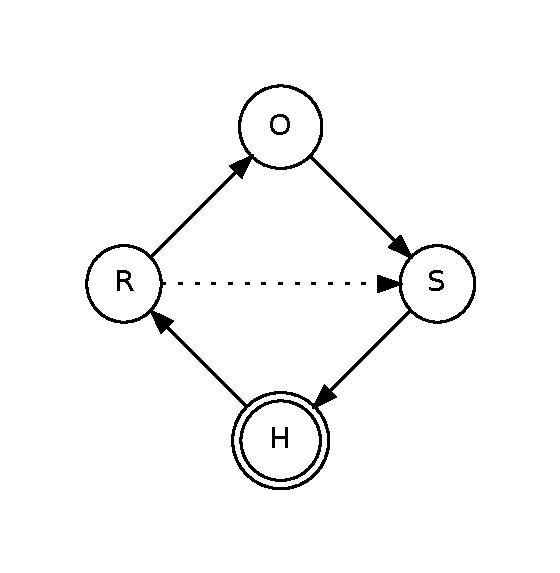
\includegraphics[scale=0.5]{states.pdf}
	\caption{State diagram for individual records.}
	\label{fig:states}
\end{figure}

The state of a resource record is defined by its reputation in 
world's caches. There are 2 certain states, \emph{Hidden} and \emph
{Omnipresent}. In the first state a resource record is not available 
in any cache (anymore). Similarly in the latter state we are sure 
all caches have a copy of the record or can at least obtain it (i.e. 
they have no old unexpired resource record set).

The two other states represent uncertainty: \emph{Rumoured} and \emph
{Squashed}. The separation is a bit artificial as they more or less 
mean the same. Both represent that some caches do and some don't 
know about the resource record. However, in our model actions (which 
are observable by the outside world) are only taken on state 
transitions. If the goal of a key changes while a record is in an 
uncertain state the records reputation does not immediately change. We 
do however must explicitly tell the component responsible for 
publishing the record to introduce or withdraw it. This transition 
is represented by the dashed arrow in Figure~\ref{fig:states}.

Since DNS involves caches and TTLs, it is entirely possible for a 
record being in the \emph{Rumoured} state while in fact every cache 
in the world holds the record. The problem is the uncertainty, we have
no way to know a record is fully propagated other than waiting the
worst case propagation time. This is also true for the \emph{Squashed}
state.

\paragraph{Summary.} A record is always in one of these four states:

\begin{description}
       \item[\emph{Hidden}:] 		
			The record is in no cache at all.
       \item[\emph{Rumoured}:] 		
			The record is published but not every cache might be aware.
       \item[\emph{Omnipresent}:]
			Every cache has this record.
       \item[\emph{Squashed}:]
			The record is withdrawn but some caches might still have it.
\end{description} 

\paragraph{Formal definition of record states.} Let $r$ be a record, $Anounced$ the 
collection of records that are actively published, and $\mathbb{C}$
the collection of all caches in the world. The states are defined by:

\begin{displaymath}
\begin{array}{lllll}
       r\in Hidden      & \equiv & H(r) &=& \forall c \in \mathbb{C} \cdot r \not \in c \\
       r\in Rumoured    & \equiv & R(r) &=& \exists c \in \mathbb{C} \cdot r \not \in c \wedge \exists c \in \mathbb{C} \cdot r\in c \wedge r\in Announced\\
       r\in Omnipresent & \equiv & O(r) &=& \forall c \in \mathbb{C} \cdot r \in c \\
       r\in Squashed    & \equiv & S(r) &=& \exists c \in \mathbb{C} \cdot r \not \in c \wedge \exists c \in \mathbb{C} \cdot r \in c \wedge r \notin Announced \\
\end{array}
\end{displaymath}

\subsection{Keyring}

Although zones can share key material the records are published 
independently. As a result each zone must have its own collection of
key states. Let us refer to this collection as a keyring denoted 
by $\mathbb{K}$. We can
define DNSSEC validity over a keyring (see Section~\ref{validity}).
It is required that every state transition of a resource record does 
not compromise the validity of the keyring as a whole.

In case a key's goal is to be \emph{Hidden} and all three involved
records are in state \emph{Hidden}, the key may be removed from the
keyring. Similar, if a key is in none of the keychains it could be
purged from the keystore.

\subsection{Key Operations}

A key and its context can be described as a tuple of states $\langle 
Ds,Dnskey,Rrsig\rangle$ for the resource records DS, DNSKEY and RRSIG.
We define the following operations on keys:

\begin{itemize}
	\item $Ds(k)$, state of DS record belonging key $k$.
	\item $Dnskey(k)$, state of DNSKEY record belonging key $k$.
	\item $Rrsig(k)$, state of RRSIG record belonging key $k$.
	\item $Goal(k) \in \{Omnipresent, Hidden\}$, the state each record
		should move towards.
	\item $Roles(k) \subseteq \{zsk,ksk\}$ excluding $\emptyset$, the 
		role(s) a key $k$ should be used for.
	\item $Alg(k)$, algorithm of key $k$ for which a transitive equivalence
		is defined.
\end{itemize}

\section{DNSSEC Validity} \label{validity}

With the definitions of Section~\ref{sec:keystates} and beyond we can
express the validity of a zone with respect to DNSSEC. After each state
transition it must still hold. If not, the zone might be treated as
\emph{bogus} by some or all validators. This check does only takes the 
total set of states in to account, it has no notion of time. It can
only guarantee every cache has a consistent view on the data when all
transitions respected the time constraint and it was ran after each
transition.

This check is not intended to be used by key management software but
functions to validate our transition model, either empirical or by 
formal proof.

\paragraph{Consistent Keys}
A consistent key is defined as a key that does not introduce 
internal inconsistencies. Additionally, a (partially) propagated KSK must have a fully
propagated ZSK.

\begin{equation}
\begin{array}{l}
ConsistentKeys \equiv \{ k | k\in\mathbb{K}, \\
\hskip 1cm	Roles(k) \subseteq {ksk} \rightarrow (\neg H(Ds(k)) \rightarrow O(Dnskey(k))) \wedge \\
\hskip 1cm	\neg H(Dnskey(k)) \rightarrow O(Rrsig(k)) \wedge \\
\hskip 1cm	( \\
\hskip 2cm		H(Dnskey(k)) \vee \\
\hskip 2cm		ksk=Roles(k) \rightarrow \exists k' \in \mathbb{K} \cdot (\\
\hskip 3cm			zsk \in Roles(k') \wedge \\
\hskip 3cm			Alg(k)=Alg(k') \wedge \\
\hskip 3cm			O(Dnskey(k')) \wedge \\
\hskip 3cm			O(Rrsig(k'))\\
\hskip 2cm		)\\
\hskip 1cm	)\\
\}
\end{array}
\end{equation}

\paragraph{Safe Keys}
SafeKeys are keys that might be internally inconsistent but for which
a consistent counterpart exists.

\begin{equation}
\begin{array}{l}
SafeKeys \equiv \{ k | k\in\mathbb{K}, \\
\hskip 1cm 		k \in ConsistentKeys \vee \\
\hskip 1cm 		\forall r \in Roles(k) \cdot ( \\
\hskip 2cm 			\exists k' \in \mathbb{K} \cdot ( \\
\hskip 3cm 				Alg(k') = Alg(k) \wedge \\
\hskip 3cm 				r \in Roles(k') \wedge \\
\hskip 3cm 				l \in ConsistentKeys \wedge \\
\hskip 3cm 				r = ksk \rightarrow (\neg H(Ds(k)) \rightarrow O(Ds(k'))) \wedge \\
\hskip 3cm 				\neg H(Dnskey(k)) \rightarrow O(Dnskey(k')) \\
\hskip 2cm 			)\\
\hskip 1cm 		)\\
\}
\end{array}
\end{equation}

\paragraph{Validity} A zone or keyring is valid if no single key 
breaks validity and at least one complete chain for any algorithm 
exists. An insecure zone is represented by a \textsc{null} key.

\begin{equation}
\begin{array}{l}
Valid(\mathbb{K}) \Leftrightarrow \\
\hskip 1cm	\forall k \in \mathbb{K} \cdot k \in SafeKeys \wedge \\
\hskip 1cm	\exists k \in \mathbb{K} \cdot ( \\
\hskip 2cm		ksk \in Roles(k) \wedge \\
\hskip 2cm		O(Ds(k)) \wedge \\
\hskip 2cm		O(Dnskey(k)) \wedge \\
\hskip 2cm		O(Rrsig(k)) \wedge \\
\hskip 2cm		\exists k' \in \mathbb{K} \cdot ( \\
\hskip 3cm			zsk \in Roles(k') \wedge \\
\hskip 3cm			O(Dnskey(k')) \wedge \\
\hskip 3cm			O(Rrsig(k')) \wedge \\
\hskip 3cm			Alg(k)=Alg(k')\\
\hskip 2cm		)\\
\hskip 1cm	)
\end{array}
\end{equation}

\section{Transition Rules}

The transition rules are explicitly written in such a way that at 
least one valid chain is being kept; a zone can not go insecure\footnote{
This prevents the system taking an 'insecure shortcut' to a new key.}. To support the insecure concept one could introduce a 
\textsc{null} key. The \textsc{null} key has it's unique (\textsc 
{null}-)algorithm. Its resource records have state but no actual 
public data. This key can be rolled in and out like any other key.

\subsection{Transition rules for $Ds(k)$}

\subsubsection*{$H(Ds(k))$}

\mathbox{
	If k is not a KSK the DS state does not matter. If is \emph{is}, before
	submitting either DNSKEY must be propagated or an other key with the 
	same algorithm should be ready.
	\begin{equation}
		\left.
		\begin{split}
			Goal(k)=O & \wedge ksk \not \in Roles(k) \\
			\\
			Goal(k)=O & \wedge O(Dnskey(k)) \\
			\\
			Goal(k)=O & \wedge 
				\exists k' \in \mathbb{K} 
				( \\
					& Alg(k)=Alg(k') \\
					& \wedge ksk \in Roles(k') \\
					& \wedge O(Ds(k')) \\
					& \wedge O(Dnskey(k')) \\
					& \wedge O(Rrsig(k')) 
				) 
		\end{split}
		\right\}\rightarrow [submit], R(Ds(k)) 
	\end{equation}
}

\subsubsection*{$R(Ds(k))$}

\mathbox{
	
	Nothing should depend on this RR yet.
	\begin{equation}
		\begin{split}
			Goal(k)=H \rightarrow S(Ds(k))
		\end{split}
	\end{equation}

	Has the user confirmed the DS is on its way to the parent and are 
	we sure everything propagated since then?
	\begin{equation}
		\left.
		\begin{split}
			Goal(k)=O & \wedge ksk \not \in Roles(k) \\
			\\
			Goal(k)=O 	& \wedge Confirmed(k_{ds}) \\
						& \wedge T_{now} \geq T_{whatever}
		\end{split}
		\right\}\rightarrow O(Ds(k))
	\end{equation}

	Postpone for later.

	\begin{equation}
		\begin{split}
			Goal(k)=O 	& \wedge Confirmed(k_{ds}) \\
						& \wedge T_{now} < T_{whatever} \\
						& \rightarrow [event]
		\end{split}
	\end{equation}
}

\subsubsection*{$O(Ds(k))$}

\mathbox{
	DS may go in State W if it refers to nothing.
	Or if there are other keys with the same algorithm which are valid.
	Or we don't break other keys and we have some other valid key(s).
	\begin{equation}
		\left.
		\begin{split}
			Goal(k)=H 	& \wedge \forall r \in Roles(k) \\
			( \\
				& \exists k' \in \mathbb{K} ( k' \not = k \\
				&\wedge Alg(k) = Alg(k') \\
				& \wedge r \in Roles(k') \\
				& \wedge O(Ds(k')) \\
				& \wedge O(Dnskey(k')) \\
				& \wedge O(Rrsig(k'))) \\
			)\\
			\\
			%~ TODO: replace forall(implication) with not exists
			Goal(k)=H 	& \wedge ksk \in Roles(k) \\
			& \wedge \forall r \in Roles(k) \\
			( \\
				& \forall k' \in \mathbb{K} ( k' \not = k \\
					& \wedge Alg(k) = Alg(k')  \\
					& \wedge r \in Roles(k') \\ 
					& \rightarrow H(Ds(k'))
				)\\
				& \wedge \\
					&\exists k' \in \mathbb{K} (k' \not = k \\
					%~ & Alg(k) \not = Alg(k') \\
					& \wedge r \in Roles(k') \\
					& \wedge O(Ds(k')) \\
					& \wedge O(Dnskey(k')) \\
					& \wedge O(Rrsig(k'))
				) \\
			)\\
			\\
			Goal(k)=H 	& \wedge ksk \not \in Roles(k) \\
				& \wedge \exists k' \not \in \mathbb{K} (k' \not = k \\
				& Alg(k) = Alg(k') \\
				& \wedge ksk \in Roles(k') \\
				%~ & \wedge State(k'_{ds}) = P \\
				%~ & \wedge O(Dnskey(k')) \\
				& \wedge \neg H(Dnskey(k')) \\
				& \wedge O(Rrsig(k'))
				)
		\end{split}
		\right\} \rightarrow S(Ds(k)) \\
	\end{equation}
}

\subsubsection*{$S(Ds(k))$}

\mathbox{

	We must wait till at least $T_{whatever}$ before transition to State 
	Ceased. As a bonus, ZSKs may transition immediately.
	\begin{equation}
		\left.
		\begin{split}
			%~ Goal(k)=H & \wedge 
			ksk \not \in Roles(k)\\
			\\
			%~ Goal(k)=H 	& \wedge 
			T_{now} \geq T_{whatever}
		\end{split}
		\right\} \rightarrow H(Ds(k))
	\end{equation}

	\begin{equation}
		\begin{split}
			%~ Goal(k)=H 	& \wedge 
			T_{now} < T_{whatever}
						& \rightarrow [event]
		\end{split}
	\end{equation}
}


\subsection{Transition rules for $Dnskey(k)$}

\subsubsection*{$H(Dnskey(k))$}

\mathbox{
	If the signatures are propagated we may submit the Dnskey. 
	Some other valid key is also acceptable.
	\begin{equation}
		\left.
		\begin{split}
			Goal(k)=O &\wedge O(Rrsig(k))\\
						&\wedge zsk \in Roles(k) \\
			\\
			Goal(k)=O & \wedge O(Rrsig(k))\\
					& \wedge \exists k' \in \mathbb{K}( \\
					& Alg(k')=Alg(k) \\
					&\wedge zsk \in Roles(k') \\
					&\wedge O(Ds(k')) \\
					&\wedge O(Dnskey(k')) \\
					&\wedge O(Rrsig(k'))) \\
			\\
			Goal(k) = O 
				&\wedge \forall r \in Roles(k) \\
				(\\
					& \exists k' \in \mathbb{K}(k' \not = k \\
					&\wedge Alg(k')=Alg(k) \\
					&\wedge r \in Roles(k') \\
					&\wedge O(Ds(k')) \\
					&\wedge O(Dnskey(k')) \\
					&\wedge O(Rrsig(k'))) \\
				)\\
		\end{split}
		\right\} \rightarrow R(Dnskey(k))
	\end{equation}
}

\subsubsection*{$R(Dnskey(k))$}

\mathbox{

	Skip the propagated state. Nobody heard of it anyway.
	\begin{equation}
		\begin{split}
			Goal(k)=H \rightarrow S(Dnskey(k))
		\end{split}
	\end{equation}

	We did wait long enough to make sure the dnskey record is known in 
	every cache?
	\begin{equation}
		\begin{split}
			Goal(k)=O \wedge T_{now} \geq T_{whatever} \rightarrow O(Dnskey(k))
		\end{split}
	\end{equation}

	We did not wait long enough: Wait some more.
	\begin{equation}
		\begin{split}
			Goal(k)=O \wedge T_{now} < T_{whatever} \rightarrow event(T_{whatever})
		\end{split}
	\end{equation}
}

\subsubsection*{$O(Dnskey(k))$}

\mathbox{

	If not part of a chain, withdraw. If there is still a DS make sure 
	there is some other valid chain for this algorithm. If none for 
	this algorithm are broken, some other algorithm will do as well.
	
	\begin{equation}
		\left.
		\begin{split}
			Goal(k)=H 
				&\wedge H(Ds(k))\\
				&\wedge H(Rrsig(k)) \\
			\\
			Goal(k)=H 
			%~ &\wedge State(k_{ds}) = C \\
				& \wedge \forall r \in Roles(k) \\
				(\\
				& \exists k' \in \mathbb{K} ( k' \not = k \\
				& \wedge Alg(k')=Alg(k) \\
				& \wedge r \in Roles(k') \\
				& \wedge O(Ds(k')) \\
				& \wedge O(Dnskey(k')) \\
				& \wedge O(Rrsig(k')) )\\
				) \\
				\\
			Goal(k)=H  &\wedge H(Ds(k))\\
				& \wedge \forall r \in Roles(k) \\
				(\\
				& \forall k' \in \mathbb{K} ( k' \not = k \\
				& \wedge Alg(k')=Alg(k) \\
				& \wedge r \in Roles(k') \\
				& \rightarrow H(Dnskey(k'))) \\
				& \wedge \\
				& \exists k' \in \mathbb{K} ( k' \not = k \\
				%~ & \wedge Alg(k') \not = Alg(k) \\
				& \wedge r \in Roles(k') \\
				& \wedge O(Ds(k')) \\
				& \wedge O(Dnskey(k')) \\
				& \wedge O(Rrsig(k')) )\\
				)
		\end{split}
		\right\} \rightarrow S(Dnskey(k))
	\end{equation}
}

\subsubsection*{$S(Dnskey(k))$}

\mathbox{

	State may transition to Ceased given enough time passed to propagate 
	change. 
	%~ Or when DS is already Ceased (only the DS is waiting this 
	%~ transition).
	\begin{equation}
		\left.
		\begin{split}
			%~ Goal(K) &=H \wedge 
			ksk \not \in Roles(k)\\
			\\
			%~ Goal(k)&=H \wedge 
			T_{now} \geq T_{whatever}
			%~ \\
			%~ Goal(k)&=C \wedge State(k_{ds})=C
		\end{split}
		\right\}\rightarrow H(Dnskey(k))
	\end{equation}

	Else, schedule event.
	\begin{equation}
		\begin{split}
			%~ Goal(k)=H \wedge 
			T_{now} < T_{whatever} \rightarrow event(T_{whatever})
		\end{split}
	\end{equation}
}

\subsection{Transition rules for $Rrsig(k)$}

\subsubsection*{$H(Rrsig(k))$}

\mathbox{
	Signatures for ZSKs can be introduced. For KSKs there must be a 
	valid ZSK.
	\begin{equation}
		%~ \left.
		\begin{split}
			Goal(k)=O 
		\end{split}
		%~ \right\} 
		\rightarrow R(Rrsig(k))
	\end{equation}
}

\subsubsection*{$R(Rrsig(k))$}

\mathbox{

Don't wait till signatures are propagated.
	\begin{equation}
		\begin{split}
			Goal(k)=H \rightarrow S(Rrsig(k))
		\end{split}
	\end{equation}

Enough time passed to propagate signatures. Or if we do a smooth 
transition 
	\begin{equation}
		\left.
		\begin{split}
			Goal(k)=O &\wedge T_{now} \geq T_{whatever} \\
			\\
			Goal(k)=O & \wedge AllowSmooth \\
					& \wedge \forall r \in Roles(k) (\\
						& \exists k' \in \mathbb{K} ( \\
							& Alg(k') = Alg(k) \\
							& \wedge r \in Roles(k') \\
							& \wedge O(Dnskey(k')) \\
							& \wedge O(Rrsig(k')) \\
						)
					)
		\end{split}
		 \right\} \rightarrow O(Rrsig(k))
	\end{equation}
	


Not enough time passed to propagate signatures.
	\begin{equation}
		\begin{split}
			Goal(k)=O \wedge T_{now} < T_{whatever} \rightarrow event(T_{whatever})
		\end{split}
	\end{equation}
}


\subsubsection*{$O(Rrsig(k))$}

\mathbox{

	If the dnskey is gone from all caches can we withdraw the 
	signatures. We may break the chain if other valid keys are 
	available.

	\begin{equation}
		\left.
		\begin{split}
			Goal(k)=H &\wedge H(Dnskey(k)) \\
			\\
			Goal(k)=H
				& \wedge \forall r \in Roles(k) \\
				( \\
				& \exists k' \in \mathbb{K} ( k' \not = k \\
					& \wedge Alg(k) = Alg(k') \\
					& \wedge r \in Roles(k')\\
					& \wedge O(Ds(k')) \\
					& \wedge O(Dnskey(k')) \\
					& \wedge O(Rrsig(k'))) \\
				)
		\end{split}
		\right\} \rightarrow S(Rrsig(k))
	\end{equation}
}

\subsubsection*{$S(Rrsig(k))$}

\mathbox{

	Dnskey is gone so no one needs these signatures.
	\begin{equation}
		\left.
		\begin{split}
			%~ Goal(k)=H &\wedge 
			H(Dnskey(k)) \\
			\\
			%~ Goal(k)=H &\wedge 
			T_{now} \geq T_{whatever} 
		\end{split}
		\right\} \rightarrow H(Rrsig(k))
	\end{equation}

	\begin{equation}
		\begin{split}
			%~ Goal(k)=H \wedge 
			T_{now} < T_{whatever} \rightarrow event(T_{whatever})
		\end{split}
	\end{equation}
}


\end{document}
